%%%%%%%%%%%%%%%
%
% $Autor: Wings $
% $Datum: 2020-01-29 07:55:27Z $
% $Pfad: Nano33BLESense.tex $
% $Version: 1785 $
%
%
%%%%%%%%%%%%%%%


%todo citatzions in correct manner
%source: {\tiny Quelle: \url{https://www.arduino.cc/pro/tutorials/portenta-h7}}



%todo GitLab\ToDo\TinyML
% TinyML Seite 222

%source: \url{https://www.reichelt.de/de/de/arduino-nano-33-ble-sense-nrf52840-ohne-header-ard-nano-33bles-p261306.html?PROVID=2788&gclid=Cj0KCQjwna2FBhDPARIsACAEc_Uui0sowk2McNvt69o9wzQJtqHWW2n5l_OHng2pSRcmfYqUsiosbdUaAp47EALw_wcB&&r=1}


\chapter{Arduino Nano 33 BLE Sense}


Arduino is an open-source electronics platform based on flexible, easy-to-use hardware and software. It provide us on board microcontroller and microprocessor kits for making digital and analogue devices. The microcontroller, oftenly called as tiny computer embed on the arduino board, normally in order to run these microcontroller we need some type of electronics e.g; diodes, resisters, capacitors, and transistors for making the voltage and current balancing. But the arduino team make a user friendly environment for getting rid of these electronics complication to run the hardware on software, just power the board as per the required voltage write the desired programm and upload it in a few seconds, it will bring everything on the board and  make us independent from any worry about the electronics complication. By the technological advancement in semiconductor and electronics  industry, the  control problems are now being solved by using these small size microcontroller instead of mechanical and electrical swithes. All Arduino boards have one thing in common which is a microcontroller, it is basically a really small computer, which help us to make a edge computing application.\cite{Arduino:2021b}
\Mynote{Advertisement! Rewrite more as an engineer!}

\section{Arduino Nano 33 BLE Sense}

The Arduino Nano Family is a set of boards with a tiny footprint, packed with features. It ranges from the inexpensive, entry model Nano , to the more feature-packed Nano BLE Sense / Nano RP2040 Connect which comprises of Bluetooth / Wi-Fi radio modules. These boards also have a set of embedded sensors, such as temperature, humidity, pressure, gesture, microphone and more. They can also be programmed with MicroPython and supports Machine Learning. \cite{Raj:2019}.

Arduino Nano 33 BLE Sense is one type of arduino family board, which is come up with Bluetooth Low Energy (BLE) capability for communication and set of sensors. This compact and reliable Nano board is built around the NINA B306 module for BLE and Bluetooth 5.0 communication; Bluetooth 5.0 is the latest version of the Bluetooth wireless communication standard. Use of microcontrollers has become inevitable in almost every field of engineering.  The Arduino Nano 33 BLE Sense module is based on Nordic nRF52480 processor that contains a powerful Cortex M4F and the board has a rich set of sensors that allow the creation of innovative and highly interactive designs. Its reduced power consumption, compared to other same size boards, together with the Nano form factor opens up a wide range of applications. 



The model name Arduino Nano 33 BLE Sense, itself puts out some important information. It is called ``Nano'' because of its compact nano size. ``33'' is included in the model name to indicate that the board operates on 3.3V.  Then the name ``BLE'' indicates that the module supports Bluetooth Low Energy and the name ``Sense'' indicates that it has on-board sensors like accelerometer, gyroscope, magnetometer, temperature and humidity sensor, Pressure sensor, Proximity sensor, Colour sensor, Gesture sensor, and even a built-in microphone. \cite{Raj:2019}.


Also, for making the RGB color and person detection, we need to make the interface of BLE 33 Sense with camera shield Arducam OV2640. The Arducam OV2640 camera use  to detect the RGB, object detetion and also the gesture too. Arduino Nano 33 BLE Sense and camera shield Arducamis a perfect match for making ML and AI application, by having the set of sensors on board we just need to install the respective library on Arduino boar and it support the funcnality of sensors and Machine learning application.
\Mynote{Advertisement! Rewrite more as an engineer!}


The following figure ~\ref{ArduinoNano33} shows a Arduino Nano 33 BLE Sense, shows how compact it is and small in size.

\begin{figure}[ht]
    \centering
    
\begin{tikzpicture}
    \ArduinoNanoTikz
\end{tikzpicture}
    
%    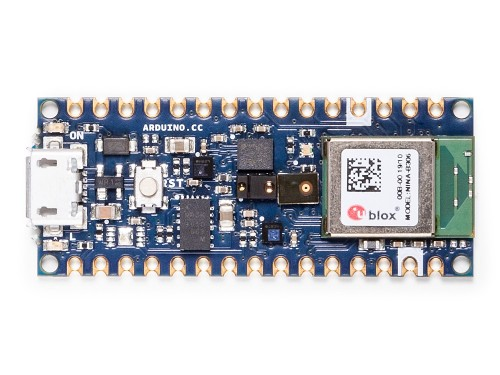
\includegraphics[width=0.45\linewidth]{Arduino/ArduinoNano33BLESense}
%    
%    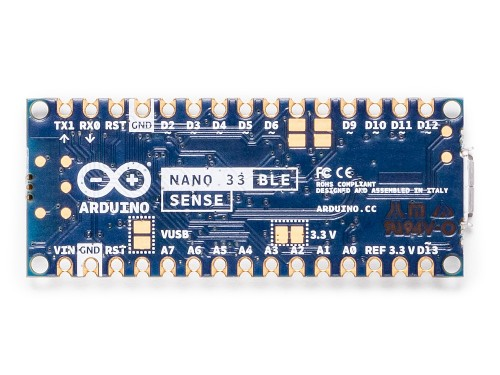
\includegraphics[width=0.45\linewidth]{Arduino/ArduinoNano33BLESense2}
% 
%    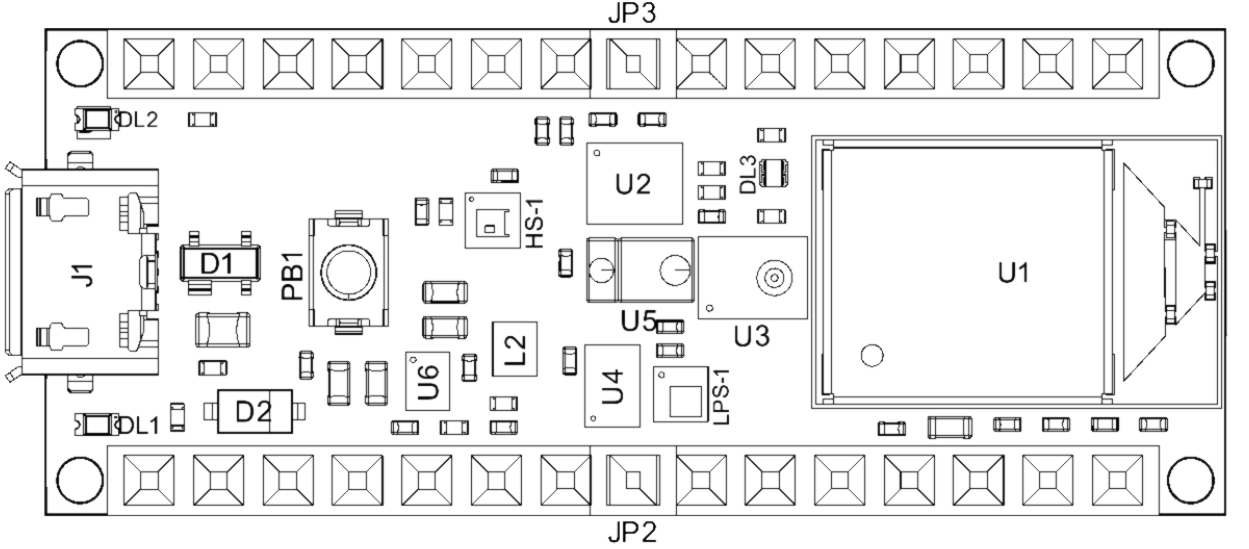
\includegraphics[width=0.45\linewidth]{Nano33BLESense/ArduinoNano33BLESenseTopology}
 
    
    \caption{Arduino Nano 33 BLE Sense, see \href{https://store.arduino.cc/arduino-nano-33-ble-sense}{Arduino Store}} 
    \label{ArduinoNano33}
    \Mynote{tikz?}
\end{figure}


The BLE (Bluetooth Low Energy) compact and reliable Nano board are built on NINA B306 module for BLE and Bluetooth 5 communication; the NINA B306 module based on Nordic nRF52480 processor that contains a powerful Cortex M4F CPU, Its architecture fully compatible with Arduino IDE Online and Offline. The Arduino Nano BLE 33 Sense have a following set of sensors on board, ADPS-9960, LPS22HB, HTS221, LSM9DS1,and MP34DT05-A. It is small in size, having all the required sensor on board. \cite{Arduino:2021}


The Arduino Nano 33 BLE Sense have the following set of Sensors, BLE module and its functionality below.

\begin{itemize}
    \item The Bluetooth is managed by a NINA B306 module.
    \item The ADPS-9960 is a digital proximity, ambient light, RGB and gesture sensor.
    \item The LSM9DS1 is a system-in-package featuring a 3D digital linear acceleration sensor, a 3D digital angular rate sensor, and a 3D digital magnetic sensor.
    \item The LPS22HB reads barometric pressure and environmental temperature.
    \item The HTS221 senses relative humidity.
    \item The MP34DT05 is support the sound detection.
\end{itemize}


\section{Unterschied zwischen dem Arduino Nano 33 BLE Sense Rev1, dem Arduino Nano 33 BLE Sense Rev2 und dem Arduino Nano 33 BLE Sense Lite}

\subsection{What is the difference between Rev1 and Rev2?}

The differences between the Arduino Nano 33 BLE Sense and the Arduino Nano 33 BLE Sense Rev2 concern the IMU, the temperature and humidity sensor, the microphone, the crypto chip and the voltage converter. In the second revision, the LSM9DS1 IMU has been replaced by two modules: the BMI270 acceleration and angular rate sensor and the BMI150 magentometer. The HTS221 humidity sensor has been replaced by the HS3003, with the latter promising greater accuracy. The values of the microphones have remained the same despite the change from the MP34DT05 to the MP34DT06JTR. Similarly, only the component designations of the voltage converters differ. The first generation uses the MPM3610, the Rev2 uses the MP2322. However, the crypto chip is no longer present in the Rev2.



\bigskip


The changes are summarized below:

\begin{itemize}
    \item Replacement of the IMU of LSM9DS1 (9 axes) with a combination of two IMUs (BMI270 - 6 axes IMU and BMM150 - 3 axes IMU).
    \item Replacement of the temperature and humidity sensor from HTS221 to HS3003.
    \item Replacing the microphone from MP34DT05 to MP34DT06JTR.
\end{itemize}

\bigskip
    
In addition, some components and changes have been made to increase user-friendliness:


\begin{itemize}
    \item Replacing the power supply from MPM3610 to MP2322.
    \item Add a VUSB solder pad to the top of the board.
    \item New test points for USB, SWDIO and SWCLK.
\end{itemize}

\bigskip

\subsection{Changes in the sketch}


For sketches that were created with libraries such as LSM9DS1 for the IMU or HTS221 for the temperature and humidity sensor, these libraries must be changed to the following for the new revision: 

\begin{itemize}
    \item Arduino\_BMI270\_BMM150 for the new combined IMU, and
    \item Arduino\_HS300x for the new temperature and humidity sensor.
\end{itemize}

\bigskip

Rev 1
\HREF{https://downloads.arduino.cc/libraries/github.com/bcmi-labs/Arduino_TensorFlowLite-1.15.0-ALPHA.zip 3}{TensorFlow Lite lib}


\subsection{Arduino Nano 33 BLE Sense Lite}


The Tiny Machine Learning Kit contains only the Arduino Nano 33 BLE Sense Lite. \Mynote{citation}

\bigskip



\bigskip

The Arduino Nano 33 BLE Sense Lite differs only slightly from the Arduino Nano 33 BLE Sense Rev2. The only difference between the two models is that the Lite version does not have the HTS221, but the LPS22HB sensor. This is a pressure sensor, but it can also be used to measure the temperature. It is therefore not possible to measure humidity with the Lite. To measure relative humidity, a separate sensor must be connected. The reason for this decision is that the Arduino company has difficulties maintaining the stock. \cite{Filipi:2022}






\section{On-Board Sensor Description}

Arduino Nano 33 BLE sense come up with the set of embed sensor on the board. The available embed sensors are commonly use for measuring both the analog and digital values around the sorrounding. Arduino Nano 33 BLE sense is very small 45mm $\times$ 18mm in size, which  makes it very usefull for Internet of things (IOT) and Artificial intelligence (AI) application as a embed device where space is the main constrained issue. It is low power consumption board and operate normally on 3.3 V, we can say that this small size low power consumption board can operate on small batteries even for many months. Due to on-board available sensor, the low power consumption and mini architecture we can use this nano board anywhere. The Arduino Nano 33 BLE Sense is a completely new board on a well-known form factor. For getting detail information about each component of Arduino Nano 33 BLE Sense and data sheets of each sensor the following links give us a detail information \cite{Arduino:2021}. The short description of each sensor are as follow. 

\begin{itemize}
    \item The ADPS-9960 is a digital proximity, ambient light, RGB and gesture sensor. it can measure the proximity distance, light, color and gestures when moving close with the borad.
    \item The sensor LSM9DS1 is a 9 axis \ac{imu} use as a accelerometre, gyroscope, and magnatometre, this 9 axis sensor is ideal for wearable devices.
    \item The sensor LPS22HB is a barometric pressure sensor, it measures the environmental pressure which is usefull for simple weather station monitoring. 
    \item The sensor HTS221 senses the relative humidity, and temperature, to get highly accurate measurements of the environmental conditions.
    \item The sensor MP34DT05 is the digital microphone. it is usefull for capturing, analyzing and detecting the sound in real time.
    \item The USB port allows you to connect  Arduino Nano 33 BLE sense to your machine.
    \item There are 3 different LEDs that can be accessed on the Nano BLE Sense: RGB Programmable LED , the built-in  orange Programmable LED and the Power LED.
    
\end{itemize}

The figure \ref{ArduinoNano33BLESenseArchitecture} show the embed sensors on the board, with powerful processor as compared to other arduino boards the nRF52840 from Nordic Semiconductors, a 32-bit ARM\textsuperscript{\textregistered} Cortex\textsuperscript{\texttrademark}-M4 CPU processor running at 64 MHz are as follow.

\begin{center}
  \begin{tikzpicture}
    \ArduinoNanoTikz
    
    \node(HTS) at (-10,5){\textcolor{red}{\tiny HTS221}};
    \draw[line width=1pt,red]  (-6.3,2.8) -- (-10,4.9);
    \node(APD) at (-6,5){\textcolor{red}{\tiny APDS9960}};
    \draw[line width=1pt,red]  (-5,2.25) -- (-6,4.9);
    \node(LSM9DS1) at (-2,5){\textcolor{red}{\tiny LSM9DS1}};
    \draw[line width=1pt,red]  (-5,3.15) -- (-2,4.9);

    \node(LSM9DS1) at (1,5){\textcolor{red}{\tiny RGB Programmable LED}};
    \draw[line width=1pt,red]  (-3.6,2.95) -- (1,4.9);
    
    \node(HTS) at (1.5,2.25){\textcolor{red}{\tiny Nordic nRF 52840}};
    \draw[line width=1pt,red]  (-2,2.25) -- (0.5,2.25);
    
    \node(MP) at (-2,-0.75){\textcolor{red}{\tiny MP34DT05-A}};
    \draw[line width=1pt,red]  (-3.9,2.25) -- (-1.75,-0.6);
    
    \node(MP) at (-6,-0.75){\textcolor{red}{\tiny LPS22HB}};
    \draw[line width=1pt,red]  (-4.5,1.0) -- (-6,-0.6);
    
    \node(LEDPower) at (-11.5,3.55){\textcolor{red}{\tiny Power LED}};
    \draw[line width=1pt,red]  (-10.8,3.55) -- (-10,3.55);
    
    \node(USB) at (-12,2.25){\textcolor{red}{\tiny Micro-USB Port}};
    \draw[line width=1pt,red]  (-11.1,2.25) -- (-10.2,2.25);
    
    \node(LEDOrange) at (-11.8,0.8){\textcolor{red}{\tiny Progammable LED}};
    \draw[line width=1pt,red]  (-10.8,0.8) -- (-10,0.8);
    
  \end{tikzpicture}
  \captionof{figure}{}\label{ArduinoNano33BLESenseArchitecture}
\end{center}

Another point to bear in mind is the overall 'trueness' of sensor readings based on where do you place the actual sensors in the environment, as this could be quite critical. The operating temperature should not exceed 85$^0$C and not lower than -40$^0$C. Other factors like humidity level and air pressure values should also be kept in check.

\begin{table}
   \begin{center}
            \begin{tabular}{llm{90mm}} 
                \textbf{\MapleCommand{MICROCONTROLLER}}  & nRF52840\\
                \textbf{\MapleCommand{OPERATING VOLTAGE}}  & 3.3V\\
                \textbf{\MapleCommand{INPUT VOLTAGE (LIMIT)}}  & 21V \\
                \textbf{\MapleCommand{DC CURRENT PER I/O PIN}}  & 15 mA \\
                \textbf{\MapleCommand{CLOCK SPEED}} & 64MHz \\
                \textbf{\MapleCommand{CPU FLASH MEMORY}}  & 1MB  \\
                \textbf{\MapleCommand{SRAM}}  & 256KB  \\
                \textbf{\MapleCommand{LED\_BUILTIN}}  & 13 \\
                \textbf{\MapleCommand{IMU (Accelerometer, Gyroscope, Magnetometer)}}  & LSM9DS1 \\
                \textbf{\MapleCommand{MICROPHONE}}  & MP34DT05 \\
                \textbf{\MapleCommand {GESTURE, LIGHT, PROXIMITY, COLOUR}}  & APDS9960 \\
                \textbf{\MapleCommand{BAROMETRIC PRESSURE}}  & LPS22HB \\
                \textbf{\MapleCommand{TEMPERATURE, HUMIDITY}}  & HTS221 \\	
            \end{tabular}
        \end{center}
    \caption{Technical Specifications of Arduino Nano 33 BLE Sense \cite{Arduino:2021}}
\end{table}

\begin{center}
  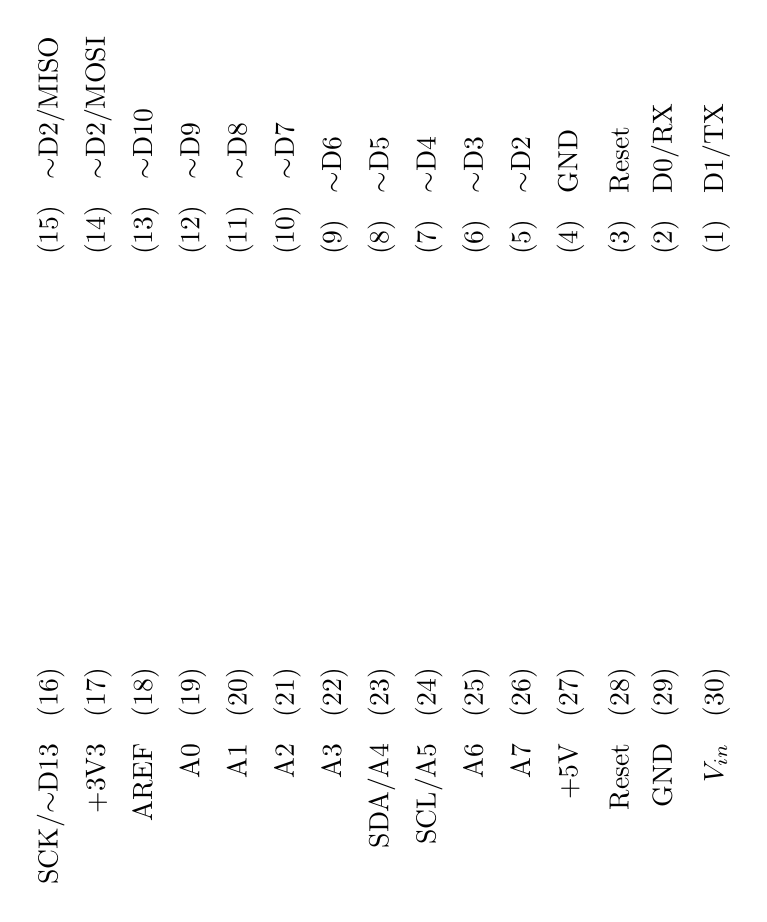
\begin{tikzpicture}
      
    \ArduinoNanoTikz

    \node[rotate=90,right] (Pin1) at (-0.91,4.6) {(1) \; D1/TX};
    \node[rotate=90,right] (Pin2) at (-1.56,4.6) {(2) \; D0/RX};
    \node[rotate=90,right] (Pin3) at (-2.11,4.6) {(3) \; Reset};
    \node[rotate=90,right] (Pin4) at (-2.76,4.6) {(4) \; GND};
    \node[rotate=90,right] (Pin5) at (-3.36,4.6) {(5) \; $\sim$D2};
    \node[rotate=90,right] (Pin6) at (-3.96,4.6) {(6) \; $\sim$D3};
    \node[rotate=90,right] (Pin7) at (-4.56,4.6) {(7) \; $\sim$D4};
    \node[rotate=90,right] (Pin8) at (-5.16,4.6) {(8) \; $\sim$D5};
    \node[rotate=90,right] (Pin9) at (-5.76,4.6) {(9) \; $\sim$D6};
    \node[rotate=90,right] (Pin10) at (-6.36,4.6) {(10) \; $\sim$D7};
    \node[rotate=90,right] (Pin11) at (-6.96,4.6) {(11) \; $\sim$D8};
    \node[rotate=90,right] (Pin12) at (-7.56,4.6) {(12) \; $\sim$D9};
    \node[rotate=90,right] (Pin13) at (-8.16,4.6) {(13) \; $\sim$D10};
    \node[rotate=90,right] (Pin14) at (-8.76,4.6) {(14) \; $\sim$D2/MOSI};
    \node[rotate=90,right] (Pin15) at (-9.36,4.6) {(15) \; $\sim$D2/MISO};
    

    \node[rotate=90,left] (Pin30) at (-0.91,-0.4) { $V_{in}$ \; (30)};
    \node[rotate=90,left] (Pin1) at (-1.56,-0.4) {GND \; (29)};
    \node[rotate=90,left] (Pin2) at (-2.11,-0.4) {Reset \; (28)};
    \node[rotate=90,left] (Pin3) at (-2.76,-0.4) {+5V \; (27)};
    \node[rotate=90,left] (Pin4) at (-3.36,-0.4) {A7 \; (26)};
    \node[rotate=90,left] (Pin5) at (-3.96,-0.4) {A6 \; (25)};
    \node[rotate=90,left] (Pin6) at (-4.56,-0.4) {SCL/A5 \; (24)};
    \node[rotate=90,left] (Pin7) at (-5.16,-0.4) {SDA/A4 \; (23)};
    \node[rotate=90,left] (Pin8) at (-5.76,-0.4) {A3 \; (22)};
    \node[rotate=90,left] (Pin9) at (-6.36,-0.4) {A2 \; (21)};
    \node[rotate=90,left] (Pin10) at (-6.96,-0.4) {A1 \; (20)};
    \node[rotate=90,left] (Pin11) at (-7.56,-0.4) {A0 \; (19)};
    \node[rotate=90,left] (Pin12) at (-8.16,-0.4) {AREF \; (18)};
    \node[rotate=90,left] (Pin13) at (-8.76,-0.4) {+3V3 \; (17)};
    \node[rotate=90,left] (Pin14) at (-9.36,-0.4) {SCK/$\sim$D13 \; (16)};

  \end{tikzpicture}
  \captionof{figure}[Pin assignment of the Arduino Nano 33 BLE Sense]{Pin assignment of the Arduino Nano 33 BLE Sense; note that the orange built-in LED is connected to pin D13 and the power LED to pin D1. The built-in RGB LED occupies pins D18, D19 and D20.}
\end{center}


\subsection{Gesture, Proximity, and Color Detection Sensor ADPS-9960}

The APDS-9960 device features advanced Gesture detection, Proximity detection, Digital Ambient Light Sense (ALS) and Color Sense (RGB). \cite{Arduino:2021} Gesture detection utilizes four directional photodiodes to sense reflected IR energy (sourced by the integrated LED) to convert physical motion information (i.e. velocity, direction and distance) to a digital information.

For the following Applications the sensor is in use:

\begin{itemize}
    \item Gesture Detection
    \item Color Sense
    \item Ambient Light Sensing
    \item Proximity Sensing
\end{itemize}

\subsection{Accelerometer, Gyroscope, and Magnetometre Sensor LSM9DS1}

The LSM9DS1 is a system-in-package featuring a 3D digital linear acceleration sensor, a 3D digital angular rate sensor, and a 3D digital magnetic sensor. \ac{imu}'s work by detecting rotational movements across the 3 axis known as Pitch, Roll and Yaw. To achieve the same, it depends on Accelerometer, Gyroscope and Magnetometer. The accelerometer gives the velocity at which the \ac{imu} module moves. The gyroscope measure the rotational movement rate on the \ac{imu}. Magnetometer measures the force of gravity acting on the \ac{imu}.

For the following Applications the \ac{imu} is in use:


\begin{itemize}
  \item Indoor navigation
  \item Advanced gesture recognition
  \item Gaming and virtual reality input devices
  \item Display/map orientation and browsing
  \item Consumer electronics; Smartphones, tablets, fitness trackers for motion sensing and orientation.
  \item Compact transportation solutions like Segway.
  \item Sports Technology - helping athletes to know how they can improve their movements.
\end{itemize}


There are also certain disadvantages of using the \ac{imu} and points that need to be kept in mind while using an \ac{imu} sensor. Accumulated error or \textit{'Drift'} is the main disadvantage of \ac{imu}s, present due to its constant measuring of changes and rounding off its calculated values off. When such a process happens for a prolonged period of time, it can lead to significant errors. The best way to avoid the \textit{drift} factor is to use a good quality \ac{imu} Sensor and make sure the \ac{imu} sensor is calibrated. \cite{STMicroelectronics:2015}
\Mynote{The explanation of drift is to small; citations}

\subsubsection{Calibration of an IMU}

\Mynote{What is calibration? citations!}

On research it was found that there are various methods to calibrate the sensors involved, the time period between each calibration is also not defined specifically, however it is advised that regular calibration is done especially when there are strange outputs noticed. Few methods of calibration are briefed below:

\subsubsection{Low and High Limit Method}

In this method the sensor is rotated in circles along each axis a few times. The midpoint is then found between the two extremes. If there is no offset, the midpoint is close to zero, but if there is a slight deviation from zero, this figure is the hard iron offset, which is the result of the distortion caused by the Earth's magnetic field. This method is mainly used to calibrate the Magnetometer \cite{Mallon:2015}

\subsubsection{Magneto V1.2}

In this method, the raw magnetometer data is pre-processed with axis specific gain correction to convert the raw output into nanoTesla: 

\begin{center} 
    
    \PYTHON{Xm\_nanoTesla = rawCompass.m.x*(100000.0/1100.0);}
    
    \PYTHON{Gain X [LSB/Gauss] for selected input field range}
    
    \PYTHON{Ym\_nanoTesla = rawCompass.m.y*(100000.0/1100.0);}
    
    \PYTHON{Zm\_nanoTesla = rawCompass.m.z*(100000.0/980.0);}
    
    
\end{center} 

This converted data is saved into the file  \FILE{Mag\_raw.txt} that you open with the Magneto program. To start using this method, we first need to replace the (100000.0/1100.0) scaling factors with values that convert your specific sensors output into nanoTesla. Rather than simply finding an offset and scale factor for each axis, Magneto creates twelve different calibration values that correct for a whole set of errors: bias, hard iron, scale factor, soft iron and misalignment.

A side benefit of this is that it can be used to calibrate accelerometers as well. You might again need to pre-process your specific raw accelerometer output, taking into account the bit depth and G sensitivity, to convert the data into milliGalileo. Then enter a value of 1000 milliGalileo as the ``norm'' for the gravitational field. \cite{Mallon:2015}




\Mynote{Here, we need more information because we want to use it:
\begin{itemize}
    \item General infomration about imus
    \item angle to roation matrix with example!
    \item calibration
    \item drift
    \item $\ldots$
    \item specials for this imu
    \item description of the parameters for coding
    \item example code, see Code/Nano33BLESense/IMU/Arduino
\end{itemize}
}

\subsection{Pressure Sensor LPS22HB}
The LPS22HB is an ultra-compact piezoresistive absolute pressure sensor which functions as a
digital output barometer.

For the following Applications the sensor is in use:



\begin{itemize}
    \item Altimeters and barometers for portable devices 
    \item Weather station equipment
    \item Sports watchs
\end{itemize}

A sensor element is installed as well as an IC interface that communicates via an I\textsuperscript{2}C or SPI bus. The function is given in a temperature range from $-40^\circ C$ to $+85^\circ C$. [STM17]

\begin{itemize}
  \item Absolutdruckbereich: 260 bis 1260 hPa
  \item Versorgungsspannung: 1,7 bis 3,6 Volt
  \item 24-bit Druckdatenausgabe
  \item 16-bit Temperaturdatenausgabe
\end{itemize}

\subsection{Relative Humidity and Temperature Sensor HTS221}
The HTS221 is an ultra-compact sensor for relative humidity and temperature. It includes a sensing element and a mixed signal to provide the measurement information through digital serial interfaces.

For the following Applications the sensor is in use:


\begin{itemize}
    \item Air conditioning, heating and ventilation 
    \item Air humidifiers
    \item Refrigerators
    \item Smart home automation
    \item Industrial automation
\end{itemize}  

Dieser Sensor kommuniziert über den I\textsuperscript{2}C- und SPI-Bus. Dieser Sensor ist einsetzbar in einem Temperaturbereich
von $-40^\circ C$ bis $+120^\circ C$. Zur Spannungsversorgung werden 1,7 bis 3,3 Volt benötigt. Eine Temperaturmessung erfolgt mit einer Genauigkeit von $\pm 5^\circ C$. [STM23]

\begin{itemize}
    \item GND - Ground
    \item DRDY - Data ready output signal
    \item SCL/SPC - I2C serial clocl (SCL) \& SPI serial port clock (SPC)
    \item VDD - Stromversorgung
    \item SDA/SDI/SDO - I\textsuperscript{2}C serial Data (SDA) \& 3 wire-SPI serial data input/output (SDI/SDO)
    \item SPI enable - I\textsuperscript{2}C/SPI mode selection
\end{itemize}

\subsection{Digital Microphone MP34DT05-A}

The MP34DT05-A is an ultra-compact, low-power, omni directional, digital microphone built with a capacitive sensing element and an IC interface. The sensing element, capable of detecting acoustic waves, is manufactured using a specialized silicon micromachining process dedicated to producing audio sensors.
The MP34DT05 is a low-distortion microphone with a signal-to-noise ratio of 64 dB. The sensitivity is -26 dBFS $\pm$ 3 dB. The \ac{aop} is 122.5 dBSPL.

The output signal of the microphone is a PDM signal. This signal is a binary signal modulated by \ac{pdm}  from the analogue signal. \cite{STMicroelectronics:2021}

For the following Applications the sensor is in use:

\begin{itemize}
    \item Speech recognition 
    \item Portable media player
    \item Mobile Terminal
\end{itemize}

\begin{figure}[h]
  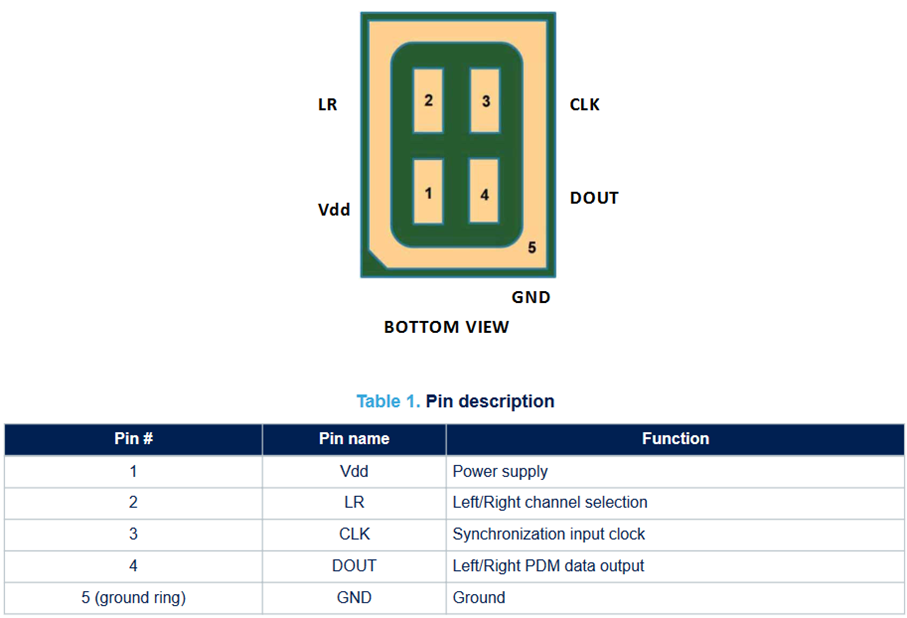
\includegraphics[width=16cm]{Microphon/MikrophonCP}
  \caption[Circuit diagram microphone]{Circuit diagram microphone \cite{STMicroelectronics:2021}}
\end{figure}

The Arduino nano 33 BLE Sense has a built-in microphone that uses PDM (Pulse-Density Modulation) to convert sound into digital data. You can use the PDM library to access the microphone data and perform various tasks with it. Here is a simple example of using the builtin microphone for an Arduino nano 33 BLE Sense:

\begin{code}
    \begin{Arduino}
        // Include the PDM library
        #include <PDM.h>
        
        // Buffer to store the microphone data
        short sampleBuffer[256];
        
        // Variable to store the sound level
        int soundLevel = 0;
        
        // Callback function for PDM data
        void onPDMdata() {
            // Read the PDM data
            int bytesAvailable = PDM.available();
            PDM.read(sampleBuffer, bytesAvailable);
            
            // Calculate the sound level
            soundLevel = 0;
            for (int i = 0; i < bytesAvailable / 2; i++) {
                soundLevel += abs(sampleBuffer[i]);
            }
            soundLevel /= bytesAvailable / 2;
        }
        
        void setup() {
            // Initialize serial communication
            Serial.begin(9600);
            while (!Serial);
            
            // Initialize PDM with a sample rate of 16 kHz and 16-bit resolution
            PDM.begin(1, 16000);
            PDM.onReceive(onPDMdata);
        }
        
        void loop() {
            // Print the sound level to the serial monitor
            Serial.println(soundLevel);
            delay(100);
        }
    \end{Arduino}
    \caption{Simple example using of the builtin microphone of the Arduino Nano 33 BLE Sense}\label{code:microphone}
\end{code}


The code~\ref{code:microphone} will print the sound level of the microphone to the serial monitor every 100 milliseconds. 

You can modify this code to perform other tasks with the microphone data, such as controlling LEDs, playing sounds, or sending data to other devices. For more information and examples, you can check out the PDM library documentation or the Arduino nano 33 BLE Sense page. 

\Mynote{How to install the library PDM\\description of the lib\\ functions}




\subsection{Bluetooth Module nRF52840}

The nRF52840 is an advanced, highly flexible single chip solution for today’s increasingly demanding Ultra Low Power (ULP) wireless applications for connected devices on our person, connected living environments and the \ac{iot} at large. It is designed ready for the major feature
advancements of Bluetooth 5 and takes advantage of Bluetooth 5's increased performance capabilities. \cite{Arduino:2021b}

\textbf{Applications}

\begin{itemize}
    \item Smart Home products
    \item Industrial mesh networks
    \item Smart city infrastructure
    \item Connected watches
    \item Advanced personal fitness devices
    \item Wearables with wireless payment
    \item Connected Health
\end{itemize}


\section{Bluetooth Module INA B306}

The module is a Bluetooth Low Energy (BLE). The connection with our smartphone is possible, to do this we have to use application ``Nordic Semiconductors nRF Connect'' They used 5.0 generation bluetooth. \ref{Figure:TestBluetoothConnect} 

\begin{center}
    \label{Figure:TestBluetoothConnect}
    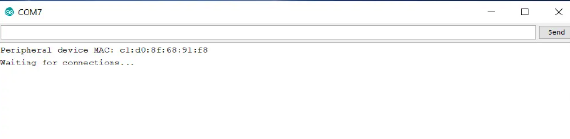
\includegraphics[width=10cm]{Bluetooth/connectionBLE.png}
    \captionof{figure}{Connection with BLE and smartphone}
\end{center}		

We can use for example to share Arduino batterie on smartphone, \ref{Code:TestBluetoothBattery} here you see an code example for how we can do this.

\begin{center}
    \captionof{figure}{Simple sketch to seen Arduino battery }
    \ArduinoExternal{}{../Code/Nano33BLESense/Bluetooth/bluetooth.ino}
    \label{Code:TestBluetoothBattery}
\end{center}




\section{Arduino Nano 33 BLE Pin Configuration}

Arduino Nano 33 BLE is an advanced version of Arduino Nano board that is based on a powerful processor the nRF52840. The figure ~\ref{Schnittstellen} shows that the board has the following pin configuration. \href{https://www.etechnophiles.com/arduino-nano-33-ble-sense-pinout-introduction-specifications/}{Pin Configuration}


\begin{description}
  \item[Digital pin] The number of digital I/O pins are 14 which receive only two values HIGH or LOW. These pins can either be used as an input or output based on the requirement. When these pins receive 5V, they are in a HIGH state and when they receive 0V they are in a LOW state.
  \item[Analog pin] Total 8 analog pins available on the board A0 -- A7. These pins get any value as opposed to digital pins that only receive two values HIGH or LOW. These pins are used to measure the analog voltage ranging between 0 to 5V.
  \item[PWM pin] All digital pins can be used as PWM pins. These pins generate analog results with digital means.
  \item[SPI pin] The board supports serial peripheral interface (SPI) communication protocol. This protocol is employed to develop communication between a controller and other peripheral devices like shift registers and sensors. Two pins are used for SPI communication i.e. Master Input Slave Output (MISO) and Master Output Slave Input (MOSI) are used for SPI communication. These pins are used to send or receive data by the controller.
  \item[I2C pin] The board carries the I2C communication protocol which is a two-wire protocol. It comes with two pins SDL and SCL.
  \item[UART pin] The board features a UART communication protocol that is used for serial communication and carries two pins Rx and Tx. The Rx is a receiving pin used to receive the serial data while Tx is a transmission pin used to transmit the serial data.
  \item[External Interrupts pin] All digital pins can be used as external interrupts. This feature is used in case of emergency to interrupt the main running program with the inclusion of important instructions at that point.
  \item[LED at Pin 13 and AREF pin] There is an LED connected to pin 13 of the board. And AREF is a pin used as a reference voltage for the input voltage.
\end{description}



\begin{figure}[ht]
    \centering
    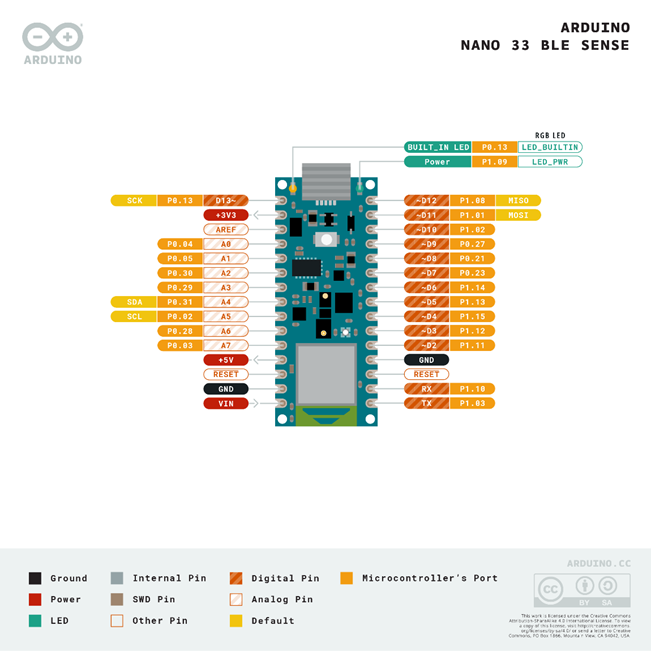
\includegraphics[width=0.5\linewidth]{Nano33BLESense/Schnittstellen}
    \caption{Arduino Nano 33 BLE Pin Configuration}
    \label{Schnittstellen}
\end{figure}


\section{\textcolor{red}{Was fehlt}}

\textcolor{red}{
\begin{itemize}
  \item Beschreibung der Sensoren
    \begin{itemize}
      \item Hintergrundwissen
      \item Beschreibung
      \item Eigenschaften
      \item Kalibrierung
    \end{itemize}
  \item Beschreibung der Bibliothek
    \begin{itemize}
      \item Beschreibung
      \item Installation
      \item Funktionen
    \end{itemize}
  \item Laufzeit, Speicherplatz, \ldots
  \item Software-Dokumentation
  \item Verwendung von Werkzeugen, z.B. Doxygen
    \begin{itemize}
      \item Beschreibung, inklusive im Quellcode; z.B. Header
      \item Handbuch
      \item Ablaufdiagramm
      \item \ldots
\end{itemize}
\item Interpretation der Ergebnisse
\item Literatur, Bilder
\item \ldots
\end{itemize}
}


